\ifdefined\beamerclass
\else
  \def\beamerclass{beamer}
\fi

\ifdefined\articlemode
	\documentclass[]{article}
	\usepackage[a4paper,margin=2cm]{geometry}
	\usepackage[envcountsect]{beamerarticle}
	\usepackage{parskip}
	\usepackage[hidelinks]{hyperref}
\else
	 \documentclass[\beamerclass,ignorenonframetext]{beamer}
\fi


\usepackage{pgfpages}
\mode<handout>{
	% \setbeamercolor{background canvas}{bg=black!20}
	\pgfpagesuselayout{2 on 1}[a4paper,border shrink=5mm]
}

\usepackage{lmodern}
\usepackage{listings}
\usepackage{amsmath}
\usepackage{bm}
\usepackage{textpos} % package for the positioning

\usepackage{pgf, tikz}
\usetikzlibrary{arrows, automata}

\usetheme{Copenhagen}
\hypersetup{pdfstartview={Fit}}
\lstset{basicstyle=\small\ttfamily,breaklines=true}

\title[Automatic Differentiation]{Automatic Differentiation (Part II)}
\author{Jonathon Hare}
\institute[]
{
  Vision, Learning and Control\\
  University of Southampton 
}
\date{}
\subject{Computer Science}
\useoutertheme{infolines}
\setbeamertemplate{headline}{} %remove headline
\setbeamertemplate{navigation symbols}{} %remove navigation symbols

\definecolor{darkblue}{RGB}{37,55,97}
\definecolor{mellowyellow}{RGB}{247,206,70}
\definecolor{almostwhite}{RGB}{254,255,255}
\definecolor{merrygreen}{RGB}{79,173,91}
\definecolor{funkyorange}{RGB}{240,154,56}

\addtobeamertemplate{footnote}{\hskip -2em}{}
\newcommand\blfootnote[1]{%
  \begingroup
  \renewcommand\thefootnote{}\footnote{#1}%
  \addtocounter{footnote}{-1}%
  \endgroup
}

\begin{document}
\mode<article>{\maketitle}

\mode<presentation>{
\begin{frame}[plain]
        \begin{tikzpicture}[overlay, remember picture, shift={(current page.south west)},font={\fontfamily{Montserrat-TOsF}\selectfont}]
        \fill [merrygreen,text=darkblue] (0,0) rectangle (\paperwidth, \paperheight);
        \draw (4,7) node [align=left,text=almostwhite] {\Huge \begin{tabular}{l} \textbf{Differentiate} \\ \textbf{Automatically} \end{tabular}};
        \draw (11,1) node [align=left,text=almostwhite] {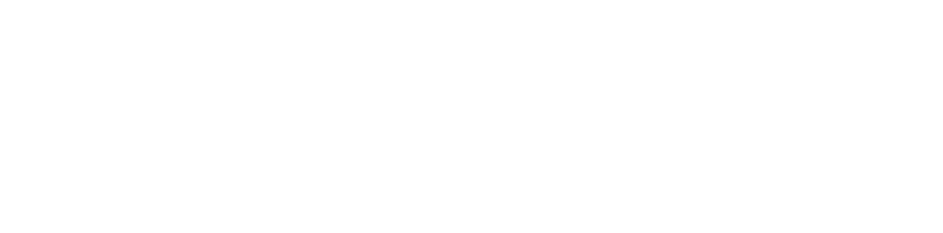
\includegraphics[scale=0.15]{../vlc.png}};
        \end{tikzpicture}
\end{frame}}

  \frame{
  \titlepage

\tiny{Much of this material is based on this blog post:
\url{https://rufflewind.com/2016-12-30/reverse-mode-automatic-differentiation}}
  }

\begin{frame}
\frametitle{What is Automatic Differentiation (AD)?}
To solve optimisation problems using gradient methods we need to compute the gradients (derivatives) of the objective with respect to the parameters.
\begin{itemize}
	\item In neural nets we're talking about the gradients of the loss function, $\mathcal{L}$ with respect to the parameters $\bm{\theta}$: 
	$\nabla_{\bm{\theta}} \mathcal{L} = \frac{\partial \mathcal{L}}{\partial \bm{\theta}}$
	\item AD is important - it's been suggested that ``Differentiable programming'' could be the term that ultimately replaces deep learning\footnote{\url{http://forums.fast.ai/t/differentiable-programming-is-this-why-we-switched-to-pytorch/9589/5}}.
\end{itemize}
\end{frame}

\begin{frame}
	\frametitle{What is Automatic Differentiation (AD)?}
	\framesubtitle{Computing Derivatives}
There are three ways to compute derivatives:

\begin{columns}
	\column{.45\textwidth}
    \setbeamercovered{transparent}
    \begin{itemize}
    	\item<1,2> Symbolically differentiate the function with respect to its parameters
    	\begin{itemize}
    		\item by hand
    		\item using a CAS
    	\end{itemize}
    	\item<1,3> Make estimates using finite differences
    	\item<1,4> Use Automatic Differentiation
    \end{itemize}

    \column{.45\textwidth}
      \begin{block}{Problems}<2>
        Static - can't ``differentiate algorithms''
      \end{block}
      \begin{block}{Problems}<3>
        Numerical errors - will compound in deep nets
      \end{block}
  \end{columns}
\end{frame}

\begin{frame}
\frametitle{Reverse Mode AD}
\begin{itemize}
	\item<+-> Whilst Forward-mode AD is easy to implement, it comes with a very big disadvantage\ldots
	\item<+-> \textbf{For every variable we wish to compute the gradient with respect to, we have to run the \emph{complete program} again.}
	\item<+-> This is obviously going to be a problem if we're talking about the gradients of a function with very many parameters (e.g. a deep network).
	\item<+-> A solution is \textbf{Reverse Mode Automatic Differentiation}. 
\end{itemize}
\end{frame}

\begin{frame}
\frametitle{Reversing the Chain Rule}

The chain rule is symmetric --- this means we can turn the derivatives upside-down:
\begin{equation*}
	\frac{\partial s}{\partial u} = \sum_i^N \frac{\partial w_i}{\partial u} \frac{\partial s}{\partial w_i} = \frac{\partial w_1}{\partial u}\frac{\partial s}{\partial w_1} + \frac{\partial w_2}{\partial u}\frac{\partial s}{\partial w_2} + \dots + \frac{\partial w_N}{\partial u}\frac{\partial s}{\partial w_N}
\end{equation*}

\uncover<2->{
In doing so, we have inverted the input-output role of the variables: $u$ is some input variable, the $w_i$'s are the output variables that depend on $u$. $s$ is the yet-to-be-given variable.
}
\\[1em]
\uncover<2->{
In this form, the chain rule can be applied repeatedly to every input variable $u$ (akin to how in forward mode we repeatedly applied it to every $w$). Therefore, given some $s$ we expect this form of the rule to give us a program to compute both $\partial s/\partial x$ and $\partial s/\partial y$ in one go\ldots
}

\end{frame}

\begin{frame}[shrink=5]
\frametitle{Reversing the chain rule: Example}

	\begin{columns}[T]
		\column{.30\textwidth}
		\begin{align*}
			\frac{\partial s}{\partial u} & = \sum_i^N \frac{\partial w_i}{\partial u} \frac{\partial s}{\partial w_i} \\[0.2em]
		x & = ? \\
		y & = ? \\
		a & = x \, y \\
		b & = \sin(x) \\
		z & = a + b
	\end{align*}
    
	\column{.6\textwidth}
	\uncover<2->{\begin{align*}
			\frac{\partial s}{\partial z} & = ? \\[0.1em]
			\frac{\partial s}{\partial b} & = \frac{\partial z}{\partial b} \frac{\partial s}{\partial z} = \frac{\partial s}{\partial z} \\[0.1em]
			\frac{\partial s}{\partial a} & = \frac{\partial z}{\partial a} \frac{\partial s}{\partial z} = \frac{\partial s}{\partial z} \\[0.1em]
			\frac{\partial s}{\partial y} & = \frac{\partial a}{\partial y} \frac{\partial s}{\partial a} = x \, \frac{\partial s}{\partial a} \\[0.1em]
			\frac{\partial s}{\partial x} & = \frac{\partial a}{\partial x} \frac{\partial s}{\partial a} + \frac{\partial b}{\partial x} \frac{\partial s}{\partial b} \\[0.1em]
			& = y \, \frac{\partial s}{\partial a} + \cos(x) \, \frac{\partial s}{\partial b} \\[0.1em]
		& = (y + \cos(x)) \, \frac{\partial s}{\partial z} \\
	\end{align*}}
	\end{columns}
\end{frame}

\begin{frame}
\frametitle{Visualising dependencies}

Differentiating in reverse can be quite mind-bending: instead of asking what input variables an output depends on, we have to ask what output variables a given input variable can affect.
\\[1em]
We can see this visually by drawing a dependency graph of the expression: \\[1em]
\begin{center}
\begin{tikzpicture}[
            shorten > = 1pt, % don't touch arrow head to node
            auto,
            node distance = 2cm, % distance between nodes
            semithick % line style
        ]

        \node[label=\footnotesize$+$] (z) {$z$};
        \node[label=\footnotesize$\sin$] (b) [above left of=z] {$b$};
        \node[label=\footnotesize$\cdot$] (a) [above right of=z] {$a$};
        \node[] (x) [above right of=b] {$x$};
        \node[] (y) [above right of=a] {$y$};

        \path[-] (z) edge node {} (a);
        \path[-] (z) edge node {} (b);
        \path[-] (b) edge node {} (x);
        \path[-] (a) edge node {} (y);
        \path[-] (a) edge node {} (x);
\end{tikzpicture}
\end{center}

\end{frame}

\begin{frame}[fragile]
\frametitle{Translating to code}

Let's now translate our derivatives into code. As before we replace the derivatives ($\partial s/\partial z, \partial s/\partial b, \dots$) with variables (\lstinline!gz, gb, ...!) which we call \emph{adjoint variables}:

\begin{lstlisting}
gz = ?
gb = gz
ga = gz
gy = x * ga
gx = y * ga + cos(x) * gb
\end{lstlisting}

\uncover<2->{
If we go back to the equations and substitute $s=z$ we would obtain the gradient in the last two equations. In the above program, this is equivalent to setting \lstinline!gz = 1!.
\\[1em]
\textbf{This means to get the both gradients $\partial z/\partial x$ and $\partial z/\partial y$ we only need to run the program once!}
}

\end{frame}

\begin{frame}
\frametitle{Limitations of Reverse Mode AD}

\begin{itemize}
	\item If we have multiple output variables, we'd have to run the program for each one (with different seeds on the output variables)\footnote{there are ways to avoid this limitation\ldots}. For example:
\[
   \begin{cases}
     z = 2x + \sin x\\
     v = 4x + \cos x
   \end{cases}
\]
	\item We can't just interleave the derivative calculations (since they all appear to be in reverse)\ldots How can we make this automatic?
\end{itemize}
\end{frame}

\begin{frame}
\frametitle{Implementing Reverse Mode AD}

There are two ways to implement Reverse AD:

\begin{enumerate}
	\item We can parse the original program and generate the \emph{adjoint} program that calculates the derivatives.
	\begin{itemize}
		\item Potentially hard to do.
		\item Static, so can only be used to differentiate algorithms that have parameters predefined.
		\item But, efficient (lots of opportunities for optimisation)
	\end{itemize}
	\item We can make a \emph{dynamic} implementation by constructing a graph that represents the original expression as the program runs.
\end{enumerate}
\end{frame}

\begin{frame}[fragile]
\frametitle{Constructing an expression graph}

\begin{columns}
	\column{.35\textwidth}

	The goal is to get something akin to the graph we saw earlier:

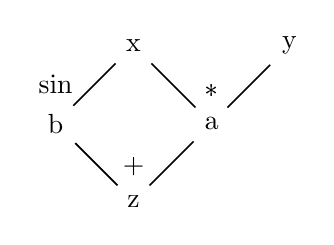
\begin{tikzpicture}[
            shorten > = 1pt, % don't touch arrow head to node
            auto,
            node distance = 1.4cm, % distance between nodes
            semithick % line style
        ]

        \node[label=\lstinline!+!] (z) {\lstinline!z!};
        \node[label=\lstinline!sin!] (b) [above left of=z] {\lstinline!b!};
        \node[label=\lstinline!*!] (a) [above right of=z] {\lstinline!a!};
        \node[] (x) [above right of=b] {\lstinline!x!};
        \node[] (y) [above right of=a] {\lstinline!y!};

        \path[-] (z) edge node {} (a);
        \path[-] (z) edge node {} (b);
        \path[-] (b) edge node {} (x);
        \path[-] (a) edge node {} (y);
        \path[-] (a) edge node {} (x);
\end{tikzpicture}

\column{.65\textwidth}

\begin{onlyenv}<2->
The ``roots'' of the graph are the independent variables \lstinline!x! and \lstinline!y!. Constructing these nodes is as simple as creating an object:

\begin{lstlisting}[language=python]
class Var:
  def __init__(self, value):
    self.value = value
    self.children = []
    ...
  ...

x = Var(0.5)
y = Var(4.2)
\end{lstlisting}
\end{onlyenv}

\uncover<3->{Each \lstinline!Var! node can have \emph{children} which are the nodes that depend directly on that node. The children allow nodes to link together in a \textbf{Directed Acyclic Graph}.}

\end{columns}

\end{frame}

\begin{frame}[fragile]
	\frametitle{Building expressions}

Each new expression $u$ registers itself as a child of each dependency $w_i$, together with the local derivative $\partial w_i/\partial u$ used during the reverse sweep:

\begin{lstlisting}[language=python]
class Var:
  ...
  def __mul__(self, other):
    z = Var(self.value * other.value)

    # weight = dz/dself = other.value
    self.children.append((other.value, z))

    # weight = dz/dother = self.value
    other.children.append((self.value, z))
    return z
  ...
...
# "a" is a new Var that is a child of both x and y
a = x * y
\end{lstlisting}
\end{frame}

\begin{frame}[fragile]
\frametitle{Computing gradients}

Finally, to get the gradients we need to propagate the derivatives. To avoid unnecessarily traversing the tree multiple times we will \emph{cache} the derivative of a node in an attribute \lstinline!grad_value!:
\begin{lstlisting}[language=python,basicstyle=\footnotesize\ttfamily]
class Var:
  def __init__(self):
    ...
    self.grad_value = None

  def grad(self):
    if self.grad_value is None:
      # calculate derivative using chain rule
      self.grad_value = sum(weight * var.grad() for weight, var in self.children)
    return self.grad_value
	...
...
a.grad_value = 1.0
print("da/dx = {}".format(x.grad()))
\end{lstlisting}
\end{frame}

% \begin{frame}
% \frametitle{Reverse Mode AD}
% \begin{block}{Let's try this for ourselves\ldots}
% \begin{itemize}
% 	\item Launch \lstinline!jupyter notebook! and load the \lstinline!ReverseAD.ipynb! notebook.
% 	\item Work through the exercises.
% \end{itemize}
% \end{block}
% \end{frame}

\begin{frame}
\frametitle{Aside: Optimising Reverse Mode AD}
\begin{itemize}
	\item<+-> The Reverse AD approach we've outlined is not very space efficient. One way to get around this is to avoid storing the children directly and instead store indices in an auxiliary data structure called a \emph{Wengert list} or \emph{tape}.
	\item<+-> Another interesting approach to memory reduction is trade-off computation for memory of the caches. The Count-Trailing-Zeros (CTZ) approach does just this\footnote{Andreas Griewank (1992) Achieving logarithmic growth of temporal and spatial complexity in reverse automatic differentiation, Optimization Methods and Software, 1:1, 35-54, DOI: 10.1080/10556789208805505}.
	\item<+-> \textbf{But,} in reality memory is relatively cheap if managed well...
\end{itemize}
\end{frame}

\begin{frame}
\frametitle{AD in the PyTorch autograd package}

\begin{itemize}
	\item<+-> PyTorch's AD is remarkably similar to the one we've just built: \begin{itemize}
		\item<+-> it eschews the use of a tape
		\item<+-> it builds the computation graph as it runs (recording explicit \lstinline!Function! objects as the children of \lstinline!Tensors! rather than grouping everything into \lstinline!Var! objects)
			\item<+-> calling \lstinline!.backward()! runs the reverse sweep and accumulates gradients for leaf tensors in their \lstinline!.grad! attributes---hence the need to call \lstinline!zero_grad()! before the next optimisation step.
	\end{itemize}
	\item<+-> PyTorch does some clever memory management to work well in a reference-counted regime and aggressively frees values that are no longer needed.
	\item<+-> The backend is actually mostly written in C++, so its fast, and can be multi-threaded (avoids problems of the GIL).
	\item<+-> It allows easy ``turning off'' of gradient computations through \lstinline!requires_grad!.
	\item<+-> In-place operations which invalidate data needed to compute derivatives will cause runtime errors, as will variable aliasing...
\end{itemize}
\end{frame}


\begin{frame}
\frametitle{Reverse mode computes a VJP}

For a function $\bm{f}:\mathbb{R}^n\rightarrow\mathbb{R}^m$, its Jacobian has shape $m\times n$.

Give the output a seed vector $\bm{v}\in\mathbb{R}^m$. A reverse sweep computes
\begin{equation*}
	\underbrace{\bar{\bm{x}}^\top}_{1\times n}
	=
	\underbrace{\bm{v}^\top}_{1\times m}
	\underbrace{\bm{J}_{\bm{f}}(\bm{x})}_{m\times n}
	\quad\Longleftrightarrow\quad
	\bar{\bm{x}}=\bm{J}_{\bm{f}}(\bm{x})^\top\bm{v}.
\end{equation*}

\begin{itemize}
	\item<2-> $\bm{v}^\top\bm{J}_{\bm{f}}(\bm{x})$ is a \textbf{vector--Jacobian product} (VJP).
	\item<3-> The adjoints propagated in our earlier program are the components of $\bar{\bm{x}}$.
	\item<4-> Reverse mode computes this product without constructing the Jacobian itself.
\end{itemize}
\end{frame}


\begin{frame}
\frametitle{The seed chooses the output combination}

\begin{block}{Cotangent vector}
	A cotangent vector is a vector of sensitivities. Applied to a small output change $\delta\bm{y}$, it gives the corresponding scalar change $\bm{v}^\top\delta\bm{y}$.
\end{block}

The output cotangent $\bm{v}$ defines a scalar function
\begin{equation*}
	s(\bm{x}) = \bm{v}^\top\bm{f}(\bm{x}).
\end{equation*}

\uncover<2->{Its gradient is exactly the VJP written as a column vector:}
\begin{equation*}
	\uncover<2->{\nabla_{\bm{x}}s
	=\bm{J}_{\bm{f}}(\bm{x})^\top\bm{v}.}
\end{equation*}

\begin{itemize}
	\item<3-> $\bm{v}=\bm{e}_i$ selects output $f_i$; $\bm{e}_i$ is all zeros except for a 1 in position $i$.
	\item<4-> An arbitrary $\bm{v}$ differentiates a weighted sum of the outputs.
	\item<5-> For a scalar output, $m=1$ and the usual seed is simply $v=1$.
\end{itemize}
\end{frame}


\begin{frame}
\frametitle{JVPs and VJPs probe different directions}

\begin{columns}
	\column{.46\textwidth}
	\begin{block}{Forward mode: JVP}<1->
		\begin{equation*}
			\bm{J}_{\bm{f}}(\bm{x})\bm{u}
		\end{equation*}
		\begin{itemize}
			\item seed an input direction $\bm{u}$
			\item one sweep per required Jacobian column
		\end{itemize}
	\end{block}

	\column{.46\textwidth}
	\begin{block}{Reverse mode: VJP}<2->
		\begin{equation*}
			\bm{J}_{\bm{f}}(\bm{x})^\top\bm{v}
		\end{equation*}
		\begin{itemize}
			\item seed an output weighting $\bm{v}$
			\item one sweep per required Jacobian row
		\end{itemize}
	\end{block}
\end{columns}

\vspace{0.5em}
\uncover<3->{\centering Deep learning usually has millions of parameters but a scalar loss: reverse mode gives the complete parameter gradient in one sweep.}
\end{frame}


\begin{frame}[fragile]
\frametitle{Computing a VJP with PyTorch}

\begin{lstlisting}
import torch
from torch.func import vjp

def f(x):
    return torch.stack((x[0] * x[1], torch.sin(x[0])))

x = torch.tensor([2., 3.])
y, vjp_fn = vjp(f, x)

v = torch.tensor([1., 0.])
(JTv,) = vjp_fn(v)
\end{lstlisting}

\begin{itemize}
	\item<2-> \texttt{y} is $\bm{f}(\bm{x})$.
	\item<3-> \texttt{vjp\_fn} maps an output cotangent to input cotangents.
	\item<4-> Here \texttt{JTv} is $\bm{J}_{\bm{f}}(\bm{x})^\top\bm{v}=[3,2]^\top$.
\end{itemize}
\blfootnote{\url{https://docs.pytorch.org/docs/stable/generated/torch.func.vjp.html}}
\end{frame}


\begin{frame}[fragile]
\frametitle{\texttt{.backward()} performs the same VJP}

\begin{lstlisting}
x = torch.tensor([2., 3.], requires_grad=True)
y = f(x)
v = torch.tensor([1., 0.])

y.backward(v)
print(x.grad)      # tensor([3., 2.])
\end{lstlisting}

\begin{itemize}
	\item<2-> The argument to \texttt{backward} is the output seed $\bm{v}$.
	\item<3-> For a non-scalar output, it must have the same shape as the output.
	\item<4-> PyTorch performs the reverse sweep and accumulates $\bm{J}_{\bm{f}}(\bm{x})^\top\bm{v}$ in \texttt{x.grad}.
\end{itemize}

\begin{block}{Different interface; same mathematics}<5->
	\texttt{torch.func.vjp} returns the VJP values; \texttt{.backward()} writes them into the gradients of leaf tensors.
\end{block}
\end{frame}


\begin{frame}[fragile]
\frametitle{A scalar loss supplies the seed for us}

\begin{lstlisting}
optimizer.zero_grad()

prediction = model(inputs)
loss = criterion(prediction, targets)

loss.backward()
optimizer.step()
\end{lstlisting}

\begin{itemize}
	\item<2-> Because \texttt{loss} is scalar, \texttt{loss.backward()} implicitly uses the seed $v=1$.
	\item<3-> The resulting VJP is the gradient of the loss with respect to every leaf parameter that contributed to it.
	\item<4-> Gradients accumulate in \texttt{parameter.grad}, so they must normally be cleared before the next step.
	\item<5-> The computation graph is freed after the reverse sweep by default.
\end{itemize}
\blfootnote{\url{https://docs.pytorch.org/docs/stable/generated/torch.Tensor.backward.html}}
\end{frame}


\begin{frame}
\frametitle{Two interfaces, one reverse-mode operation}

\begin{columns}
	\column{.46\textwidth}
	\begin{block}{\texttt{torch.func.vjp}}<1->
		\begin{itemize}
			\item functional: returns values
			\item makes the cotangent explicit
			\item composes with other function transforms
			\item useful for analysis and higher-order methods
		\end{itemize}
	\end{block}

	\column{.46\textwidth}
	\begin{block}{\texttt{Tensor.backward()}}<2->
		\begin{itemize}
			\item imperative: updates \texttt{.grad}
			\item scalar losses default to seed 1
			\item gradients accumulate at leaves
			\item the standard training interface
		\end{itemize}
	\end{block}
\end{columns}

\begin{alertblock}{The common idea}<3->
	Both propagate an output cotangent backwards through the computation graph to evaluate a VJP.
\end{alertblock}
\end{frame}


% \begin{frame}
% \frametitle{Reverse Mode AD}
% \begin{block}{Let's try this for ourselves\ldots}
% \begin{itemize}
% 	\item Launch \lstinline!jupyter notebook! and load the \lstinline!PyTorchAD.ipynb! notebook.
% 	\item Work through the exercises.
% \end{itemize}
% \end{block}
% \end{frame}

\end{document}
